\documentclass[crop,tikz]{standalone}
\usetikzlibrary{shapes}
\usetikzlibrary{arrows}
\usetikzlibrary{positioning}

\begin{document}
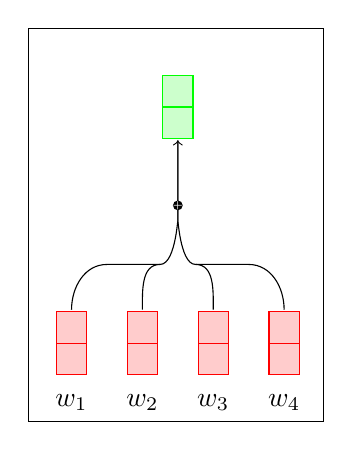
\begin{tikzpicture}[
  hid/.style 2 args={
    rectangle split,
    draw=#2,
    rectangle split parts=#1,
    fill=#2!20,
    outer sep=.25mm},
  mlp/.style 2 args={
    rectangle split,
    rectangle split horizontal,
    draw=#2,
    rectangle split parts=#1,
    fill=#2!20,
    outer sep=.25mm}
]

 % Comment out this line to remove border.
 \draw[draw=black] (0, 5) rectangle (3.75, 0);

 \foreach \step in {1,...,4} {
   \node (i\step) at (.9*\step -.35, .25) {$w_\step$};
   \node[hid={2}{red}] (e\step) at (.9*\step - .35, 1) {};    
 }
 
 \node[hid={2}{green}] (s) at (.9 * 2.5 - .35, 4) {};
 \draw[->] (e1.north) to [out=90,in=180] (1.35 - .35, 2) 
    to (.9 * 2.25 - .35, 2)
    to [out=0,in=90] (.9 * 2.5 - .35, 2.5) to (s.south);
 \draw[-] (e4.north) to [out=90,in=0] (.9 * 3.5 - .35, 2) 
    to (.9 * 2.75 - .35, 2)
    to [out=180,in=90] (.9 * 2.5 - .35, 2.5) to (s.south);

 \draw[-] (e3.north) to [out=90,in=0] (.9 * 2.75 - .35, 2) ;
 \draw[-] (e2.north) to [out=90,in=180] (.9 * 2.25 - .35, 2) ;

   \node[circle,fill,inner sep=1.25pt] (t) at (.9*2.5 - .35, 2.75) {};
   \node[white] (p) at (.9*2.5 - .35, 2.75) {\scalebox{.4}{\textbf{+}}};
 
\end{tikzpicture}
\end{document}
